
% CHAPTER 1

\chapter{INTRODUCTION}
\label{chp:introduction}

This thesis work focuses on dynamic adaptation to achieve changes in formation of swarms consisting of heterogeneous mobile robots. The term of swarm has a meaning \cite{4}, a large group of locally interacting individuals with common goals. 

Self organizing swarm researches and its applications are generally inspired from the biological systems existing in the nature. Behaviours of complex biological systems remained unresolved for a long time, until recent researches that showed individuals with supple functionalities can achieve complex tasks by cooperation \cite{2}. Biological systems (such as colonies of ants) have simple behaviours but they can accomplish very complicated collective tasks in nature quite impossible to be achieved solely by individual capabilities. Beni \cite{1} describes this collaboration of members as follows:

Collaborative robot network is not just a agglomeration of robots, they have essential characteristics, which are found in swarms of insects, that is, decentralised control, which does not require synchronisation, and individuals which are simple and (quasi) identical.

Properties of swarm robotics systems that make them unique are the simplicity of individuals, restricted sensing and communication capabilities, collaborative achievement of complex tasks, robustness and decentralization of control capabilities \cite{6}.

Swarm robotics has been studied to produce different collective behaviours to solve tasks such as as aggregation , pattern formation , self-assembly and morphogenesis , object clustering, assembling and construction , collective search$\&$rescue and exploration , coordinated motion , collective transportation , self-deployment , foraging and others\cite{5}. Dorigo and Trianni \cite{7} are studied on controllers for aggregation of coordinated motion of the identical mobile robots called swarm-bots. Their implementation has a centralized structure in which a decision maker assigns roles to individual agents. In our work, each agent is responsible to reach global consensus on the final positions in formation which increase the robustness of the system against to individual erroneous decisions. Hou, S.P., C.C. Cheah, and J.J.E. Slotine is focused on controlling of a swarm within a dynamically changing formation \cite{8}. In their work, it is needed to describe a global objective function which requires analytical expression of the desired formation shape. But it may not be possible to define the desired formation shape with analytical expressions in real world applications. In this thesis work, the solution does not require the analytical expressions of the desired formation shape.  Ganesh and Lisa introduced two new strategies for collective search and exploration of fields with swarm intelligence \cite{9}. Their implementation requires a central controller to manage the individuals and this type of solution has a single point of failure characteristic because of the dependence on single decision maker agent.   Chaimowicz and Campos proposed a new methodology which is based on a dynamic role assignment mechanism in which the robots cooperate with each other and they demonstrate this method in a cooperative transportation task \cite{10}. Their work implements a leader follower structure in which following agents has no impact on the global consensus of the swarm. This approach depends on the decision of an individual agent and an erroneous decision of this individual may cause the failure of whole swarm. 

There are lots of studies related with different problems in swarm robotics literature as discussed briefly. In this thesis project, we are focused on dynamic pattern formation control of swarms consist of heterogeneous robots. All agents contribute on the decision process and they collaborate to minimize the total displacement while achieving the desired formation shape. 

\section{Problem Definition}
In this thesis work, it is aimed to design a formation control system with heterogeneous robots with dynamically changing complex shapes. Desired formation shapes for real time applications, such as covering an area or a search$\&$rescue operation, may not be simple geometrical shapes with analytical expressions. The solution which does not require a mathematical definition of the desired formation shape is more suitable for these type of applications. On the other hand, this formation shape may be dynamically changing to meet the requirements of the task in real time. 

In literature, formation control systems generally include a decision making process which is executed by an individual agent or a central server. This kind of approach creates a single point of failure system and this ruler may cause a failure for the whole swarm by making a mistake. In this work, it is aimed to implement a solution in which each member of the swarm contributes on the decisions and global consensus of the swarm.

Formation control systems which are implemented with swarms composed of homogeneous agents cannot achieve special tasks which requires different functionalities of individual agents. In this work, we have focused on implementing a solution with a swarm consisting of heterogeneous agents with different capabilities. 

In this work, the main idea is to propose a complete design solution to a dynamically changing formation system, including a local positioning and formation control system. Formation control system heavily depends on the position data of individual agents in the environment. Since it is expected to have high number of agents in the environment due to the nature of a swarm, the agents are assumed to have simple structures with low capabilities including lack of certain types of sensors. On the other hand, for indoor applications it will not be possible to use satellite dependent positioning systems on agents \cite{19}. Even if a positioning solution provided for an indoor application by different methods including visual feedback(by image processing), RSS(received signal strength) etc. , it is not possible to implement this solution for each single agent in the environment due to the increasing complexity and the costs by the number of agents. In literature, formation control systems are generally designed with the assumption of the positions of each agent is known exactly. To propose a complete solution for the formation control problem, it is required to implement a localization solution for the agents to provide the corrected positions in the workspace which will be used by the formation control system. This localization process implements a solution to correct the position data of the agents with the determined process period and within an maximum error bound. This error bound is determined by the requirements of the formation control problem. 

\section{Motivation}
The formation control problem is defined as the collaboration of a group of agents towards maintaining a formation with a certain shape \cite{12}. It focuses on leading the individual agents of a swarm to perform  collective tasks including shape generation and formation reconfiguration while traversing a trajectory avoiding collisions. These kind of tasks are achieved with a large group of small and simple robots  that can cooperate with each other. Formation control of multi agent systems  is an actively growing research field.

Swarms which are used in formation control systems, can be composed of homogeneous or heterogeneous agents according to the requirements of the problem. The usage of the homogeneous agents increases the total impact and the coverage of the system in the environment. This kind of a swarm has an increased redundancy and is capable of resuming the current task in case of failures of some of the agents during mission. On the other hand, a swarm composed of heterogeneous agents has different capabilities of the agents. This kind of a system can be used in tasks which requires different functionalities has to be performed individually or simultaneously.

In real world applications there may be need for different  functionalities to achieve some specific tasks. If this is the case, one solution may be to design a sophisticated robot which includes all required capabilities for this task. In this scenario, this robot will be the single point of failure in the system and if robustness is a  vital feature for this solution, some redundant robots have to be added to the system. It is clear that the design of such an advanced robot and hold its redundant backups in the system will increase the cost of the solution. In swarm robotics concept, one of the approaches related with the usage of the heterogeneous agents is to gather some different types of simple mobile robots which have their own specific functionalities to achieve a collective task rather than designing an advanced robot for the solution \cite{99}. With this approach, the robustness of the system is increased, costs are reduced down and the reusability of the individual members of the swarm for other tasks is provided.  A project named Swarmanoid which is funded by European Commission, has an objective to implement and control of a novel distributed robotic system. The system is designed with heterogeneous, dynamically connected, small autonomous robots called,  foot-bots , hand-bots and eye-bots where foot-bots are responsible to transport the required materials(including other types of robots) to a specific task area and foot-bots are responsible for operations to be handled with their manipulators and eye-bots are responsible of observations and reconnaissance on the area. This project implements a system which has a leader follower structure in which a decision maker agent assign different tasks and roles to the other members of the swarm. Wrong decisions or the failure of this decision maker may prevent the whole swarm to achieve the desired task. In this thesis work, we have focused on a system in which each agent is responsible to contribute on the decision process.

\begin{figure}[H]
\caption{A Robot Team Consists of Eyebot, Handbot and Footbot Agents \cite{99}}
\centering
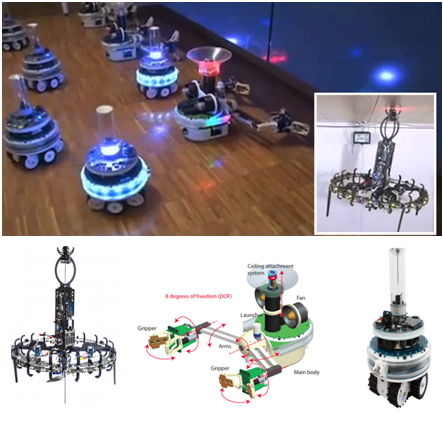
\includegraphics[scale = 1]{eyebot}
\end{figure} 

A swarm which is composed with same type of homogeneous agents can be used to increase the total impact and the energy of an individual agent. This kind of a system can be used in missions like coverage, search and  reconnaissance etc.  Martin and Kilberg have worked on formation control and formation tracking of  microsatellites to achieve continuous coverage and improved capability. They also mentioned that small formations will reduce the fuel consumption for propulsion and expand the sensing capabilities of microsatellites \cite{15}.

\begin{figure}[H]
\caption{Sparse Aperture Formation of Micro Satellites \cite{15}}
\centering
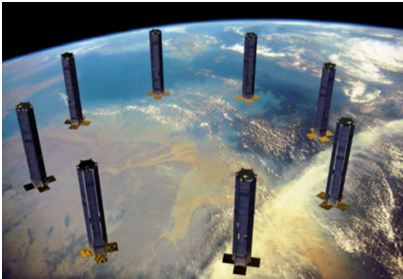
\includegraphics[scale = 1]{Satellite}
\end{figure} 

Formation control solutions has lots of usage areas such as coverage missions, security patrols and search$\&$rescue in hazardous environments etc.\cite{13}. For missions related with area coverage and reconnaissance, a group of autonomous vehicles may be required to keep in a specified formation \cite{13}.  

There are some hardware implementations to test the related formation control algorithms in real time applications. Since the formation control problem requires lots of agents in a swarm, these works have a common point of providing agents with minimal costs and sensor capabilities. The Kilobot Project from Harvard university have released their agents with the name of Kilobots and they have teams which are working on different formation control problems with Kilobots \cite{98}.

\begin{figure}[H]
\caption{Formation Control with Kilobots \cite{98}}
\centering
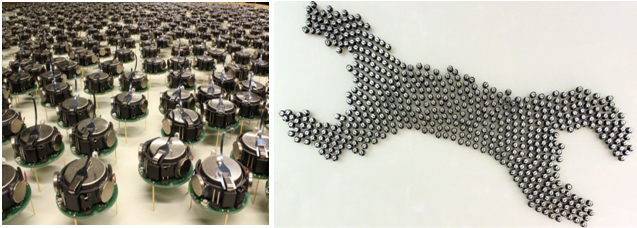
\includegraphics[scale = 0.70]{kilobot}
\end{figure}

These micro robots have a great reusability for different types of formation control problems  and they have biological inspiration from the nature in the sense of individual simplicity and power of collective behaviours. Common feature of these projects, they implement formation control systems with swarms composed of homogeneous agents. In real world applications, complex tasks may require different functionalities which can be provided by different type of robots. In our work, we have focused on implementing a formation control system with heterogeneous agents.

\begin{figure}[H]
\captionsetup{format=hang,justification=centerfirst}
\caption{
A) Swarm Robot Project from Universities of Stuttgart \cite{97}  \\
B) Colias Project from Lincoln University and Tsinghua University\cite{96}\\
C) Marx bot developed at EPFL\cite{95} \\
D)Swarm bots project conducted by  European Commission \cite{94}}

\centering
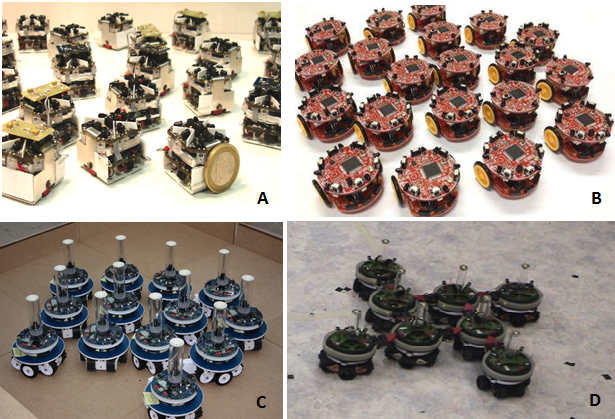
\includegraphics[scale = 0.7]{mobilerobots}
\end{figure}

    
    
  
    
Hou, S.P., C.C. Cheah, and J.J.E. Slotine has implemented a formation control system with dynamically changing formation shapes \cite{8}. Their approach defines a global objective function which requires the mathematical definition of the desired formation shape, but in real world applications it may not be possible to derive the analytical expressions for the desired shape. In our work, control laws for individuals in the swarm does not require such a global objective function definition.

\begin{figure}[H]
\caption{Dynamically Changing Formations with Global Objective Functions \cite{8}}
\centering
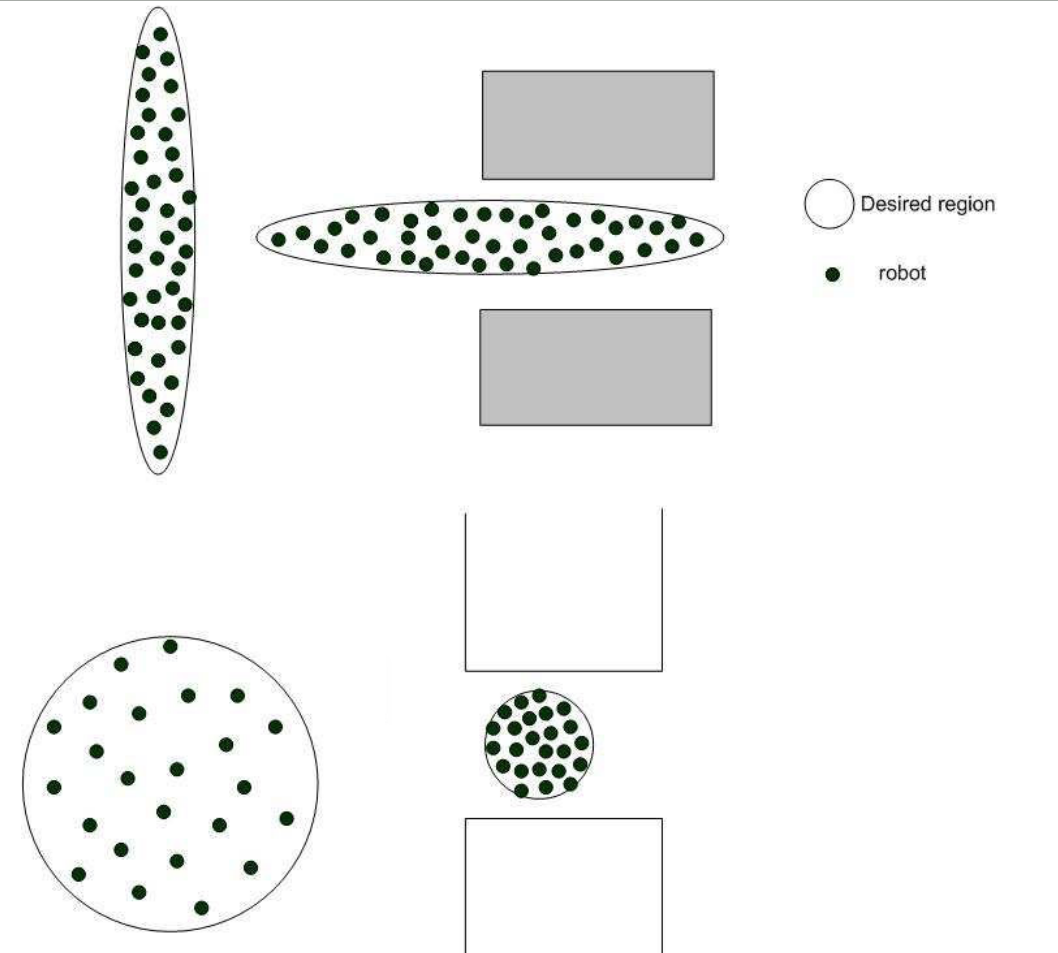
\includegraphics[scale = 0.32]{houslotine}
\end{figure}


\section{Objectives $\&$ Goals} \label{Objectives}
In this thesis work, our aim is to provide different approaches $\&$ solutions to the requirements in formation control problem.  There are mainly different types of  infrastructures which propose solutions to the formation control problems like the heterogeneity vs. homogeneity of the agents, communication structures, centralized vs. decentralized structures, swarm control strategies like behaviour based and leader-following approaches or virtual structure based approaches. 

Our main approach is to design a complete solution to the formation control problem by taking into account the requirements related with real world applications. In literature, formation control systems generally implements solutions with simple geometrical shapes \cite{8}. One of the objectives of this thesis work is to implement a solution which does not require the mathematical definition of the desired formation shape. Also it is aimed to design an algorithm which can adapt itself to the dynamically changing formations.

On the other hand, most of the related work assumes that it is possible to measure the exact positions of the agents in the workspace \cite{98,97}. Another objective of this thesis work is to implement a localization solution for the agents by assuming they may not able to measure their positions. With this approach, it is possible to provide a complete solution to formation control problem.

Specific tasks including different missions, requires agents with different capabilities and this kind of tasks may not be achieved with swarms composed of homogeneous agents \cite{99}. In our work, one of the objectives is to implement a formation control system with heterogeneous agents. Furthermore, proposed solutions for formation control problem generally includes a decision making process which is executed by an individual agent or a central server. This kind of approach creates a single point of failure system and if this decision maker unit fails during mission, swarm cannot achieve the desired task. In this thesis work, it is aimed to implement a solution in which every agent is responsible of contributing on decisions and reaching a global consensus. 

In addition to choice of the formation control infrastructures, capabilities of the individual agents provide additional requirements and constraints while designing a formation control system. One of the most important characteristic of an agent in the swarm is its simplicity and limited sensor $\&$ communication capability \cite{6}. This approach results from the idea of achieving collective tasks with lots of simple individuals  and it is based on biological inspirations in nature like colonies of ants etc. In our work, it is aimed to propose a solution by taking into account that agents in the swarm has simple structures and limited sensor capabilities.

To achieve these objectives and meet these requirements, the goals for this thesis work are defined as follows:

\subsection{Heterogenous Robots with Different Dynamics}
It is aimed to create a formation control system with heterogeneous agents to achieve complex tasks which require different functionalities. To accomplish this objective, it is assumed that agents have different dynamics from each other like different friction surfaces, geometrical structures and functionalities. They have different volumes and masses(not mass point particles) and they may collide with the other ones and the obstacles in the environment.


\subsection{Communication Infrastructure}
One of the objectives in this work is to implement a localization solution for the agents. Also it is required to implement a communication backbone to execute a decentralized decision making process in which each agent reaches a global consensus. To meet these requirements, it is needed to implement a communication infrastructure in the proposed solution. By taking into account that the agents in the swarm have limited communication capabilities and can only negotiate with its local neighbors in a narrow line of sight range due to power consumption issues and their weak radio links, this infrastructure must have following specifications.

\begin{figure}[H]
\caption{Radio Links on Agents Have a Narrow LOS Range}
\centering
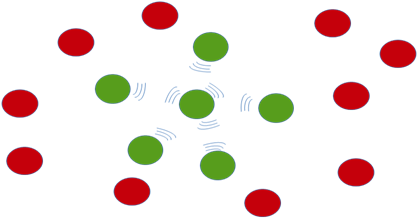
\includegraphics[scale = 1]{narrow_los}
\end{figure}

a)Communication Topology \newline
Communication topology is a wireless mesh network in which each agent relays data for the rest of the network. The network is fully connected and has routing technique where the data is propagated along a route by transporting over the nodes(member agents of the swarm).

\begin{figure}[H]
\caption{Mesh Network Between Agents}
\centering
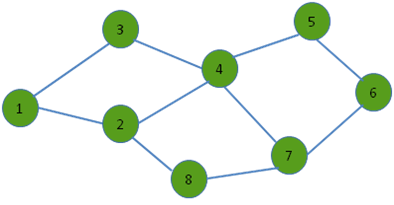
\includegraphics[scale = 1]{mesh}
\end{figure} 

b)Communication Bandwith \newline
Bandwidth of the communication between agents is limited and nodes can only transport most critical data like heartbeats, agent IDs, type and position etc.

\subsection{ Decentralized Decision Making Process}
Centralized formation controller systems implement a single controller  server/root node
to process all the data needed to achieve the desired control objectives. This type of systems achieve superior performance and optimal decisions  but they require high computational power, high communication bandwidths and are not robust due to dependence on a single controller \cite{12}. Decentralized formation controller structures have agents which are completely autonomous and responsible their own individual decisions. In this work, a hybrid centralized/decentralized controller architecture in which there is a central manager which partitions the desired formation shapes into goal states and there are independent agents who make their own choices on these goal states to reach as unaware of the other agents' choices.

\begin{figure}[H]
\caption{Agents make their own choices about target goal states}
\centering
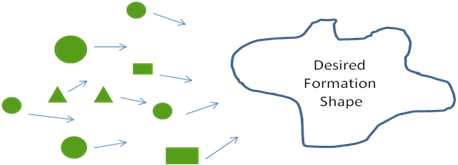
\includegraphics[scale = 0.9]{decentralized}
\end{figure} 

\subsection{Complex and Dynamically Changing Formation Shapes}
In literature, formation control systems are generally designed with a single or combination of simple geometrical shapes and they require analytical expressions of these shapes while implementing the proposed control laws for individual agents \cite{93}. Specific tasks which requires more complex shapes cannot be achieved with this approach. In our work, we have focused on designing a formation control algorithm which does not require the mathematical definition of the desired formation shape. The goal to accomplish this objective is to design a solution which does not depend on the analytical expression of the formation shape. Furthermore, in literature the general approach is to implement a solution to cover a static formation shape. In real world applications it may be needed to update the desired shape according to the requirements of the task. In our work, one of the goals is to propose an algorithm which can adapt itself to dynamically changing formation shapes.

\begin{figure}[H]
\caption{Complex and Dynamically Changing Formation Shapes}
\centering
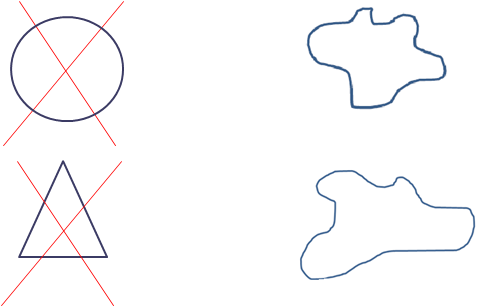
\includegraphics[scale = 1]{complex}
\end{figure}

\subsection{Simple Agents with Low Sensor Capabilities and Low Computing Powers}
Agents in the swarm are assumed to have low sensor capabilities and weak computing power \cite{6}. This condition must be taken into account during the control system design, since individuals do not have a high resolution and sensitive data about their states, and they cannot execute high level complex control algorithms.

\section{Requirements}
The goals of this project define some requirements about the implementation phase of the project. These requirements are listed as follows:

1. Agents have to propagate their position and velocity states with the help of inertial measurements.This process is handled with a Kalman estimator which takes the translational acceleration data as an input to the observer model .The translational acceleration data is calculated with the help of AHRS system composed by 3 axis accelerometers, gyroscopes and magnetometers. 

2. Agents have to update$\&$adjust their position data with the help of agents which have positioning sensors(position beacons) by local trilaterations.This position data is used in the internal estimator systems as external measurements to correct the drifts caused by propagation error of translational accelerations.  The ordering for this trilateration process have to determined appropriately to minimize the error on calculated position data of agents which are far away from the position beacons.

3. Agents have to update their route tables to create a communication backbone with the mesh network topology. Since agents are assumed to have low range$\&$bandwidth radio links, the propagation of a data between each agent in the swarm will be handled over this mesh network. 

4. Agents have to determine the goal states in the desired complex formation shape to cover with the help of a central server. Desired formation shape will be partitioned into potential goal states assigned to different types of agents. Performance analysis on proposed shape partitioning methods have to be done with some different criterias. 

5. Assignment of the agents to their target goal states should be handled to minimize the total displacement of the agents while travelling towards the desired formation shape. 

6. Simulations should be performed to compare the efficiency of different methods proposed in this thesis work. Different types of agents have to be represented with different dynamical and physical models during simulations.

7. Hardware demonstrations should be performed to illustrate the applicability of the proposed solution in real time systems. These applications may not contain the full implementation of the proposed system, but they must demonstrate a proof of concept(POC) environment.

\section{Methodology}
During the first part of the project, a local positioning system(LPS) is designed. In this system, agents which does not have position sensors propagate their position and velocity states with their inertial measurements. Due to the bias and drift errors on this solution, a position update$\&$adjust process is handled with the help of position beacons which are agents with position sensors on their boards in the swarm. During the update phase of the solution, route tables for individual agents are determined with the help of Graph Theory based Destination-Sequenced Distance Vector Routing Protocol (DSDV) algorithms. This process provides the required information to compose the clusters around position beacons and provides rank information for the agents which are in same clusters. Position measurements are handled with local trilateration process in a turn with the rank values for every agent around each cluster after the establishment of route tables. A Kalman estimator system is designed to fuse these propagation and update phases of the solution.

On the second part of the thesis work, formation controller system is designed with two novel methods based on bubble packing method and randomized fractals method. Desired complex formation shapes are partitioned into goal states according to the heterogeneous agents in the swarm for both of these two methods. Decision process of the agents about their target goal states to optimize the overall utility of the swarm is implemented with the help of Visibility Graphs and Hungarian algorithms. Internal velocity controllers for individual agents to reach the desired target goal states by providing obstacle avoidance, are implemented with a full state feedback method by regulating the augmented dynamical system with the gains optimized by Linear Quadratic Regulators (LQR).

\section{Contribution of Thesis}
The main contributions of thesis are:

1. Designing a local positioning system(LPS) based on local trilaterations to provide high accuracy position data to the agents which do not have a specific position sensors on their boards.

2. Implementing a wireless mesh network between agents in the swarm and design a communication infrastructure and related routing algorithms to exchange the local data globally in the network

3. Implementing a formation control system with complex and dynamically changing formation shapes by using swarms composed of heterogeneous agents.

4. Designing and implementing the rules$\&$algorithms for the decentralized decision making process of the individual agents about the goal states in desired formation shape.


\section{Outline of the Thesis}
This thesis work is organized into 5 main sections .Chapter 1 introduces the main theme and the potential areas of the usage of formation control, while specifying our motivation and the requirements$\&$problems to meet$\&$solve related with the topic.

Chapter 2 gives literature reviews about the related works and basic mathematical background on the methods used in this paper.

Chapter 3 introduces the methods and solutions used in two different parts of the problem; local positioning system and formation control system. In this chapter, routing algorithms and mathematical aspects of the trilateration process is introduced. Methods$\&$algorithms used for formation control is discussed in details.

Chapter 4 provides simulation analysis on the local positioning system and gives mutual evaluations of the performances of different methods used in formation control system.

Chapter 5 provides and discuss the details of hardware implementations and the experimental results.

Chapter 6 concludes the thesis and defines the future works related with the thesis.